\documentclass[12pt]{article}
\usepackage[right=2cm,left=2cm,top=2cm,bottom=3cm]{geometry}
\usepackage[utf8]{inputenc}
\usepackage[spanish]{babel}
\usepackage{amsmath}
\usepackage{color}
\usepackage{listings}
\usepackage{graphicx}
%\usepackage{multicol}

%COLORES CODIGO
\definecolor{gray97}{gray}{.97}
\definecolor{gray75}{gray}{.75}
\definecolor{gray45}{gray}{.45}
\definecolor{claregreen}{RGB}{4,180,95}
\definecolor{darkblue}{rgb}{0.0,0.0,0.6}


\lstset{ frame=Ltb,
     framerule=0pt,
     aboveskip=0.5cm,
     framextopmargin=3pt,
     framexbottommargin=3pt,
     framexleftmargin=0.4cm,
     framesep=0pt,
     rulesep=.4pt,
     backgroundcolor=\color{gray97},
     rulesepcolor=\color{black},
     %
     stringstyle=\ttfamily,
     showstringspaces = false,
     basicstyle=\small\ttfamily,
     commentstyle=\color{gray45},
     keywordstyle=\bfseries,
     %
     numbers=left,
     numbersep=15pt,
     numberstyle=\tiny,
     numberfirstline = false,
     breaklines=true,
   }

% minimizar fragmentado de listados
\lstnewenvironment{listing}[1][]
   {\lstset{#1}\pagebreak[0]}{\pagebreak[0]}

%LENGUAJE OZ
\lstdefinelanguage{OZ}
{
  morestring=[b]',
  morecomment=[s]{\%}{\%},
  stringstyle=\color{claregreen},
  keywordstyle=\color{blue}\bfseries,
  morekeywords={proc, end, \$},% list your attributes here
  emph={REQUIRED},
  emphstyle=\color{red}
}

%MODO CONSOLA
\lstdefinestyle{consola}
   {basicstyle=\scriptsize\bf\ttfamily,
    backgroundcolor=\color{gray75},
   }




%opening
\title{Simulación de Eventos Discretos.\\ \emph{Informe de Modelo e Implementación.} \\ \textbf{Simulación de Fallas de Máquinas.} }
\author{\textbf{María Andrea Cruz Blandón  0831816.} \\ \textbf{Edgar Andres Moncada 0832294.  }\\ \textbf{Luis Felipe Vargas Rojas 0836342. }}
\date{\today}







\begin{document}
\maketitle

\section{Análisis del Sistema y del Problema.}
\subsection{Descripción del Sistema}
El sistema esta compuesto de un conjunto de máquinas que funcionan en una fábrica, entre las cuales no existe conexión de manera que cada una trabaja independientemente de las otras; estas se mantienen encendidas 8 horas del día, es decir que el rendimiento total semanal se calcula con la fórmula $8*5*50$ donde 8 son las  horas del día, 5 son los días de la  semana, y 50 es el número de máquinas que están laborando.\\

Dentro de la fábrica se cuenta con un conjunto de máquinas adicionales que son enviadas a trabajar si alguna de las máquinas presenta una falla. También se cuenta con personal de mantenimiento que se encargan de reparar las máquinas que fallen; cada empleado puede reparar una máquina al tiempo, en caso de no tener a algún empleado disponible se debe poner en espera la máquina que falló, y en el momento de que un empleado la repare ésta se convierte en una máquina adicional.


\subsection{Descripción Gráfica del Sistema}
\begin{center}

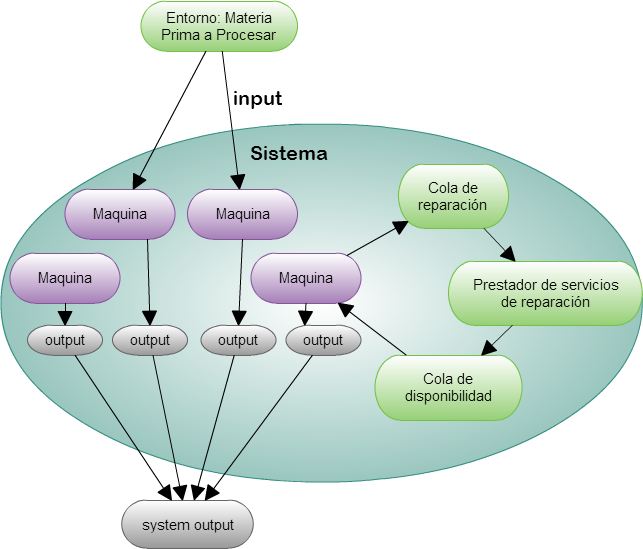
\includegraphics[scale=0.47]{Simulacion.png}

Figura1. \emph{Comportamiento del Sistema}
\end{center}

\subsection{Descripción del Problema}

La fábrica quiere mantener el stock de maquinaria principal en funcionamiento continuo por lo menos en un 96\% o 98\%. El problema que se tiene es que las máquinas son componentes que pueden presentar fallas, y estas afectan de manera general a la producción de la fábrica.\\

Para solucionar este problema la fábrica ha dispuesto de máquinas adicionales dispuestas a reemplazar las máquinas que se dañen durante el proceso, que tienen a fallar luego de $160\pm30$ horas. También se cuenta con un equipo de mantenimiento que puede reparar, las máquinas que se dañen, en aproximadamente $8\pm3$ horas. Sin embargo no siempre son suficientes las máquinas auxiliares y la cantidad de personal para atender las máquinas que fallan y mantener la utilidad requerida de funcionamiento de las 50 máquinas. Por esta razón la fábrica quiere determinar cuántas máquinas adicionales y cuánto personal es el necesario para cumplir la meta.

\section{Modelo de Simulación.}

\subsection{Simulación en general}

Puntos claves:
\begin{itemize}
\item Se debe trabajar con una lista de eventos futuros.
\item Cada máquina de la fábrica tiene la probabilidad de fallar en un periodo de $160\pm30$ horas con una distribución uniforme.
\item Una vez un reparador inicia la repación de una máquina esta reparación puede tomarle $8\pm3$ horas con una distribución uniforme.
\item La cantidad de reparadores puede variar según los escenarios planteados.
\item La cantidad de máquinas adicionales puede variar según los escenarios planteados.
\item Es adecuado realizar un tiempo de calentamiento ya que existe formación de colas.
\item Una máquina que se esté reparando o esté esperando para ser reparada no puede generar un evento de fallo, pues no está en funcionamiento. 
\end{itemize}


Al iniciar la simulación se genera un evento de fallo por cada una de las máquinas de la fábrica. Estos eventos se generan con un  espacio de $20$ horas. Esto es con el fin de evitar la situación: \emph{Todas las máquinas fallan a la vez}. Una vez se tiene este conjunto de eventos, se realiza el período del calentamiento,este consiste en realizar las acciones seg\'un el evento siguiente en la lista de eventos futuros hasta cumplir un tiempo, el cual hemos determinado 30 semanas, durante el calentamiento las variables de desempeño no están activadas, pero si se tiene en cuenta las colas y estados de éstas. Alcanzado este tiempo de calentamiento se activan las variables de desempeño, se usan las colas tal cual quedaron y se realizan las acciones pertinenetes seg\'un el tiepo de evento que se extraiga de la lista de eventos futuros esto se realiza por un tiempo $t$ que se establezca para análisis del sistema. Al finalizar se debe calcular la función de costo y realacionarla con las variables de desempeño para poder comparar dicha simulación con otros escenarios.\\

Se determinó un tiempo de 30 semanas desarrollando el siguiente análisis. Las máquinas tienen un evento de fallo que se produce una vez estén activas en una distribución uniforme de $160\pm30$ horas lo que es equivalente a $4\pm0.75$ semanas (tener encuenta que una semana corresponde al trabajo de $8*5$  horas). Dado los primeros $50$ eventos de fallo generados al iniciar la simulación, estos se generaron con un espacio de $20$ horas lo que es equivalente a $0.5$ semanas. Ahora bien $50*0.5$ siendo $50$ la cantidad de eventos y $0.5$ el tiempo con el que se generan los eventos (en semanas), nos da $25$ semanas para que posiblemente se halla ejecutado el último de los $50$ eventos generados al principio, sin embargo para extenderlo y tener seguridad de su ejecución se suman $5$ semanas más al tiempo de calentamiento quedando finalmente en $30$ semanas, esta extención de tiempo también da la oportunidad que se hallan creado una cantidad suficientes de eventos tanto de falla como de reparación. Así pues tendrémos un sistema estable el cual analizar. A continuación se presentan dos gr\'aficas donde se ve como con el calentamiento el sistema se estabiliza y sus respectivas simulaciones ya con el sistema estable.\\

\newpage

\begin{figure}
  \centering
	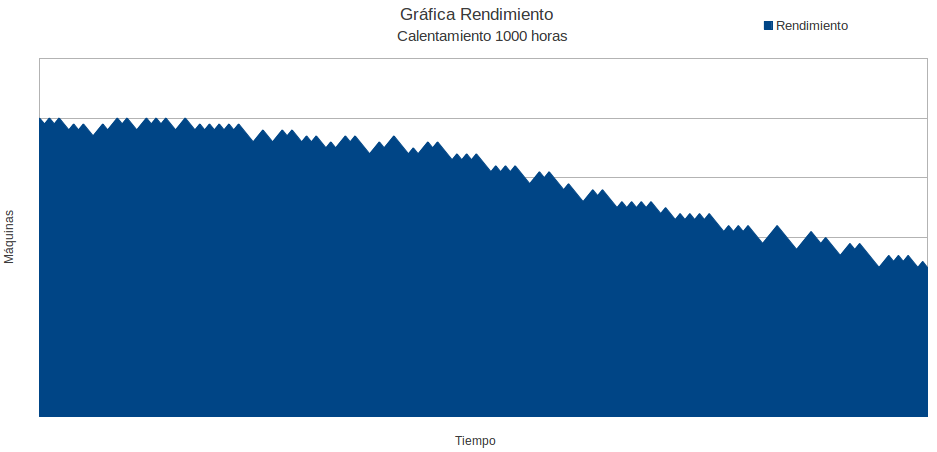
\includegraphics[scale=0.6]{graf1.png} 
  \caption{Calentamiento con m\'aximo de tiempo $1000$}
  \label{fig:cal1}
\end{figure}

\begin{figure}
  \centering
	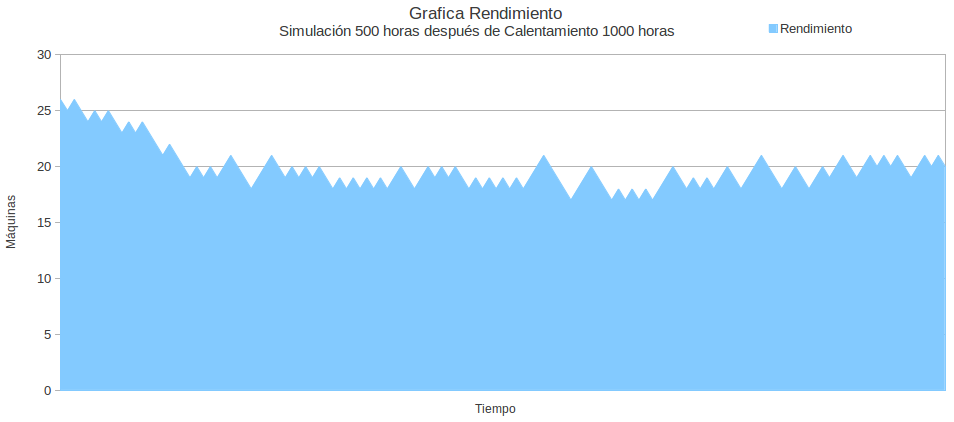
\includegraphics[scale=0.6]{graf2.png} 
  \caption{Simulaci\'on despu\'es del calentamiento de $2000$ horas de tiempo $500$}
  \label{fig:descal1}
\end{figure}

\begin{figure}
  \centering
	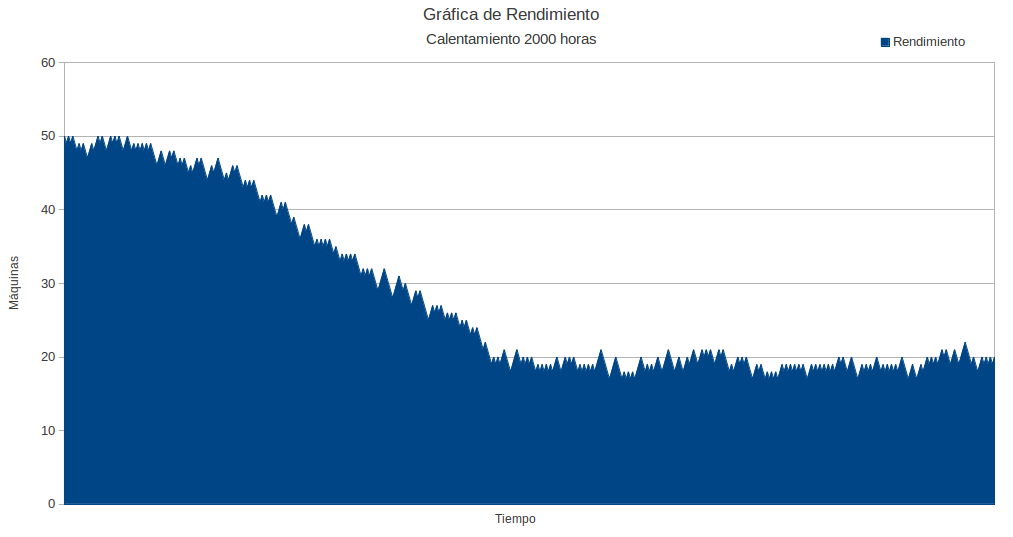
\includegraphics[scale=0.6]{graf3.png} 
  \caption{Calentamiento con m\'aximo de tiempo $2000$}
  \label{fig:descal2}
\end{figure}

\begin{figure}
  \centering
	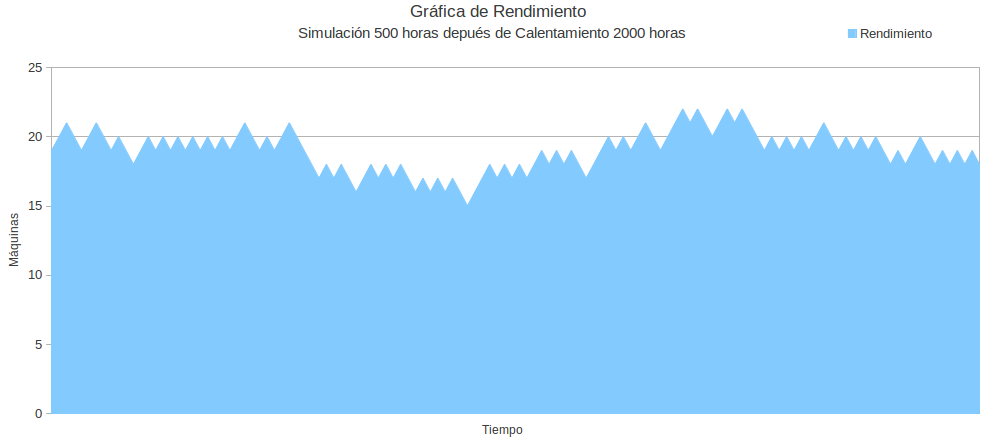
\includegraphics[scale=0.6]{graf4.png} 
  \caption{Simulaci\'on despu\'es del calentamiento de $2000$ horas de tiempo $500$}
  \label{fig:cal2}
\end{figure}

\newpage



Con el tiempo de calentamiento lo que se busca es crear un ambiente donde las colas y eventos ya estén más estables para ahí si calcular las variables de desempeño. También se busca eliminar el sesgo que ocasionan las observaciones en tiempo de transición del modelo (Cuando se inicia una simulación sin tiempo de calentamiento). \\


A continuación se muestra un diagrama de flujo de la simulación en general.\\

\begin{figure}
  \centering
    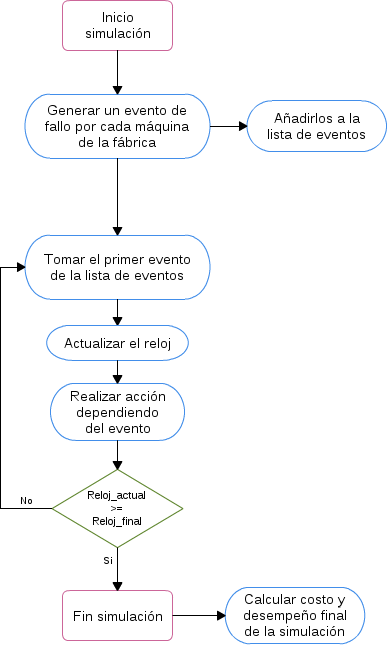
\includegraphics[scale=0.6]{Simulacion_flujo.png}
  \caption{Diagrama de flujo de la simulacin en general.}
  \label{fig:simulacion}
\end{figure}

\newpage 


\subsection{Eventos.}

Según la describción de la simulaci\'on en general, se identificaron dos eventos estos son:

\begin{enumerate}
\item \textbf{Fallo de una máquina.}\\
Cuándo una máquina falla se debe verfificar si existe máquina adicional que la reemplace para no perdudicar el rendimiento de la fábrica, si existe tal máquina que la pueda reemplazar entonces el número de m\'aquinas adicionales diminuye en uno y se genera un evento de fallo para la m\'aquina que asumi\'o el puesto, esta acci\'on tambi\'en afecta la variable de desempeño de la cola promedio de m\'aquinas adicionales; sino es as\'i se disminuye en uno la cantidad de m\'aquinas que est\'an trabajando en la f\'abrica esto afecta la variable de desempeño de rendimiento de la f\'abrica. \\

Lo siguiente es verificar si hay disponible un reparador para iniciar la reparaci\'on, si es as\'i el reparador inicia la repaci\'on y se genera el evento de repaci\'on correspondiente a dicha m\'aquina, tambi\'en se debe disminuir el n\'umero de reparadores disponibles, esta acción afecta la variable de desempeño relacionada con el promedio de ocupación de los reparadores. Si no hab\'ia reparadores disponibles, la m\'aquina debe pasar a la cola de reparaci\'on y esperar hasta poder ser reparada, la cola de repaci\'on aumenta en una unidad adem\'as esta acci\'on afecta la variable de desempeño relacionada con la cola de reparaci\'on promedio.


\item \textbf{Reparación de una máquina.}\\

Cuando una m\'aquina ha sido reparada se debe verificar si hay una estaci\'on para reemplazar en la f\'abrica, si es as\'i esta m\'aquina reasume y se genera su correspondiente evento de fallo, se aumenta en uno la cantidad de máquinas que están funcionando, además esto afecta la variable de desempeño relacionada con el desempeño de la fábrica; sino había una estación que reasumir, la máquina pasa a la cola de máquinas adicionales y ésta acción afecta la variable de desempeño relacionada con la cola promedio de la cola de máquinas adicionales.\\

Lo siguiente a verificar es si existen m\'as m\'aquinas para ser reparadas, si es así se inicia la reparaci\'on con la m\'aquina que sigue en ser reparada y se genera un evento de reparaci\'on relacionado con dicha m\'aquina, esta acci\'on afecta la variable de desempeño relacionada con la cola promedio de reparaci\'on. Sino hab\'ia m\'as m\'aquinas para ser reparadas se aumenta en uno la cantidad de reparadores disponibles y se afecta la variable de desempeño relacionada con el promedio de ocupación de reparadores.

\end{enumerate}


Diagramas de flujo de los eventos:

\newpage 

\begin{figure}
  \centering
  	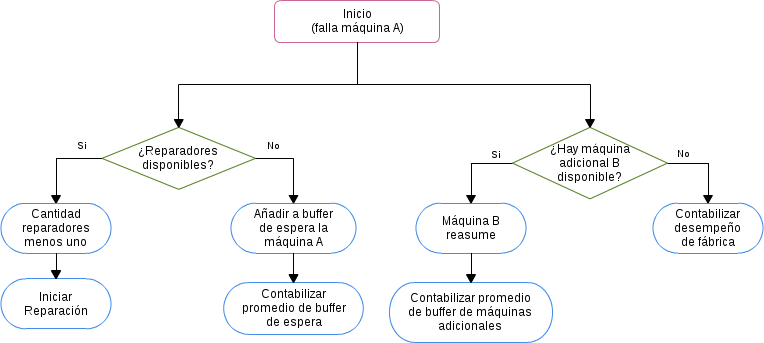
\includegraphics[scale=0.5]{EventoFallo.png} 
  \caption{Evento: Se presenta una falla en una de las máquina.}
  \label{fig:eventofallo}
\end{figure}

\begin{figure}
  \centering
  	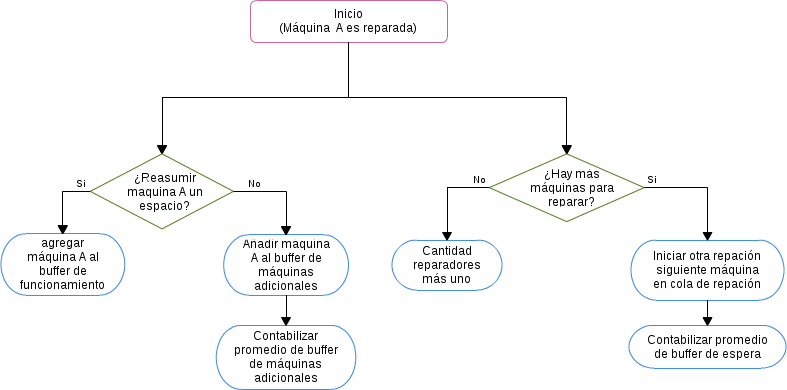
\includegraphics[scale=0.5]{EventoReparacion.png} 
  \caption{Evento: Se realiza la reparación de una de las máquinas dañadas.}
  \label{fig:eventoreparacion}
\end{figure}




\subsection{Reloj de La Simulación}

La unidad de tiempo que se va a emplear es la hora. El reloj va a avanzar de acuerdo al modelo de simulación LEF, donde se almacenan los tiempos de los eventos futuros y se ordenan cronológicamente, así el cambio de estado del reloj  se va a dar por el tiempo del evento más próximo en cada iteración.\\

La simulación termina cuando:
\begin{enumerate}
\item El reloj del sistema a llegado a un valor indicado (tiempo final).
\item No hay mas eventos futuros en la lista de eventos.
\end{enumerate}

\subsection{Comportamiento de los Datos.}

\begin{itemize}
\item \textbf{Tiempo entre los fallos de una m\'aquina}\\
El tiempo en que ocurre un evento de falla sigue una distribución uniforme $160\pm30$ horas, es decir,  $U(130,190)$.

\item \textbf{Tiempo duraci\'on reparaci\'on de una m\'aquina}\\
El tiempo que dura una repaci\'on sigue una distribuci\'on uniforme $8\pm3$ horas, es decir, $U(5,11)$.

\end{itemize}



\section{Diseño y Analisis de Escenarios.}

\subsection{Escenario: B\'asico}

Para este escenario se utiliza un solo reparador y ninguna máquina adicional. Se realiza con un tiempo de calentamiento de $1200$ horas y el tiempo tomado en cuenta en la simulación es de $500$. Se realiza $1000$ simulaciones donde se varia la semilla para luego sacar un promedio en el desempeño del funcionamiento de la fábrica.

\subsection{Escenerio: An\'alisis m\'aquinas adicionales}

Para este escenario se utiliza un solo reparador y las máquinas adicionales empiezan a añadirse. Se realiza con un tiempo de calentamiento de $1200$ horas y el tiempo tomado en cuenta en la simulación es de $500$. Se realiza $1000$ simulaciones donde se varia la semilla para luego sacar un promedio en el desempeño del funcionamiento de la fábrica. Se repiten en total $n*1000$ simulaciones donde $n$ es la cantidad de máquinas adicionales que se van a añadir.

\subsection{Escenario: An\'alisis cantidad reparadores}

Para este escenario se varia la cantidad de reparadores y con una u otro valor fijo de máquinas adicionales. Se realiza con un tiempo de calentamiento de $1200$ horas y el tiempo tomado en cuenta en la simulación es de $500$. Se realiza $1000$ simulaciones donde se varia la semilla para luego sacar un promedio en el desempeño del funcionamiento de la fábrica. Se repiten en total $n*1000$ simulaciones donde $n$ es la cantidad de reparadores que se van a añadir.

\subsection{Escenario: An\'alisis combinatoria m\'aquinas adicionales y cantidad reparadores}

Para este escenario se varia la cantidad de reparadores y máquinas adicionales. Se realiza con un tiempo de calentamiento de $1200$ horas y el tiempo tomado en cuenta en la simulación es de $500$. Se realiza $1000$ simulaciones donde se varia la semilla para luego sacar un promedio en el desempeño del funcionamiento de la fábrica. Se repiten en total $m*n*1000$ simulaciones donde $n$ es la cantidad de reparadores que se van a añadir y $m$ es la cantidad de maquinas adicionales que se vana ir añadiendo.


\subsection{Pruebas}

\section{Implementación del Modelo.}

\subsection{Estructura de datos}
\begin{itemize}

	 \item \textbf{Eventos}\\
	 Para los eventos se uso un template 
	 \begin{verbatim}
	 Evento<Tiempo, Tipo, Maquina>
	 \end{verbatim}
	 Con esta estructura de evento se tiene información necesaria para realizarle el seguimiento a la máquina, recordemos que todas las m\'aquinas tienen las mismas probabilidades de fallar pero estas son posibles en la medida que la m\'aquina est\'e funcionando. 
	 
	 \item \textbf{Lista de eventos futuros}\\
	 Para la lista de eventos futuros se utilizó la estructura \emph{Priority Queue} de java, a la cual se le debi\'o implementar la interfaz de comparaci\'on. Pues como se sabe los eventos no eran estructuras b\'asicas de java. La comparaci\'on era dado dos eventos se determinaba cual era el menor usando el tiempo de cada evento y comparando cual era el menor, este era el factor de organizaci\'on. 
	 
 	 \item \textbf{Colas}\\
 	 \begin{itemize}
 	 \item \textbf{Cola máquinas adicionales}
 	 Para llevar el conteo cada paso del reloj, se usó un entero que era afectado según el evento y estado del sistema.\\
 	 Para saber que máquina reasumia cuando se requeria se creó una estructura FIFO \emph{Queue} de java, en la cual las máquinas cuando eran reparadas ingresaban y cuando eran necesarias se sacaban para que entraran a reemplazar siguiendo la regla \emph{primeras en entrar primeras en salir}.
 	 
 	 \item \textbf{Cola espera para reparación}
 	 En este caso tambi\'en se us\'o un entero para contabilizar como cambiaba la cola de espera para reparaci\'on. \\
 	 
 	 Para saber que m\'aquina segu\'ia para ser reparada se us\'o una estructura FIFO \emph{Queue} de java, lo que se buscaba con esta estructura era que las m\'aquinas no esperaran tanto para ser reparadas y que todas sean reeparadas.
 	 \end{itemize}
 	 
 	 \item \textbf{Variables de desempeño}\\
 	 Para estas variables se usaron doubles y se iban actualizando de acuardo a lo planteado en la descripción de eventos. Usamos para calcular el promedio el área bajo la curva.
 	 
 	 \begin{figure}
 	  	\centering
 	   		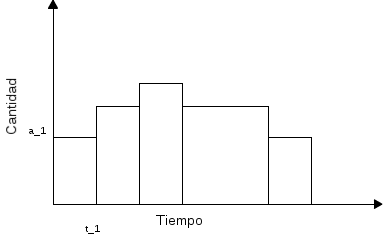
\includegraphics[scale=0.5]{promedio.png} 
     	\caption{Calculo promedio, \'area bajo la curva.}
  		\label{fig:promedios}
 	 \end{figure}
 	 
 	 En el ejemplo de la Figura \ref{fig:promedios} consiste en hallar el área de cada cuadrado y sumarlos luego se divide por el $100\%$ este puede ser, por ejemplo en el desempeño de la f\'abrica  $50*$Reloj\_Final.
 	 
\end{itemize}


\section{Conclusiones.}

En el problema de las fallas de las máquinas se puede ver como el sistema en un largo periodo de tiempo llega a estabilizarse o a tomar valores muy parecidos o a descender muy lentamente; esto en el caso de que la fábrica solo tenga inicialmente un reparador, esto se debe al largo tiempo que puede tener una maquina antes de fallar comparado con el tiempo de reparación.\\

Viendo el comportamiento del sistema, se puede ver que aumentando la cantidad de reparadores, el rendimiento de la fábrica mejora considerablemente, al contrario del aumento de máquinas adicionales que solo afectan muy poco el rendimiento.\\

Las m\'aquinas adicionales no afectan fuertemente pues ellas también fallan con la misma distribución uniforme que las m\'aquinas de la f\'abrica. Si estas tuvieran un tiempo posible de fallo mucho más grande que las m\'aquina de la fábrica tal vez representarían una mejora en el rendimiento. La m\'aquinas adicionales tambi\'en se encolan esperando para ser atendidas por los reparadores.



\end{document}

